\documentclass[11pt]{beamer}
\usetheme{Madrid}
\usefonttheme{serif}
\definecolor{customcolor}{RGB}{52,25,100} 
\setbeamercolor{structure}{fg=customcolor}

\usepackage[utf8]{inputenc}
\usepackage[T1]{fontenc}
\usepackage{amsmath}
\usepackage{amsfonts}
\usepackage{amssymb}
\usepackage{graphicx}
\usepackage{algorithm}
\usepackage{algpseudocode}
\usepackage{geometry}

\DeclareMathOperator{\sen}{sen}
\DeclareMathOperator{\tg}{tg}

\setbeamertemplate{caption}[numbered]

\author[Atishaya Maharjan]{Atishaya Maharjan}
\title{Geometric Spanning Trees and Hypergraphs that Minimizes the Wiener Index}
\newcommand{\email}{maharjaa@umanitoba.ca}
\setbeamertemplate{navigation symbols}{} 
\institute[]{University of Manitoba\par Geometric, Approximation, and Distributed Algorithms (GADA) lab} 
\date{\today} 

\bibliographystyle{apalike}

\begin{document}

\begin{frame}
	\titlepage
\end{frame}

\section{Geometric Spanning Trees and Hypergraphs that Minimizes the Wiener Index}

\begin{frame}{Wiener Index in Graphs}
	\begin{itemize}
		\item Let $G = (V, E)$ be a weighted undirected graph and let $\delta_G(u, v)$ denote the \textbf{shortest (minimum-weight) path}  between vertices $u$ and $v$ in $G$.
		      \pause
		\item The Wiener index is defined as:
		      \[
			      W(G) = \sum_{u, v \in V} \delta_G(u, v)
		      \]
		      \pause

		\item We can also equivalently define it as:
		      \[
			      W(G) = \sum_{1 \leq i < n} dist(v_i, v_{i+1}) \cdot i \cdot (n - i)
		      \]
	\end{itemize}
	\begin{center}
		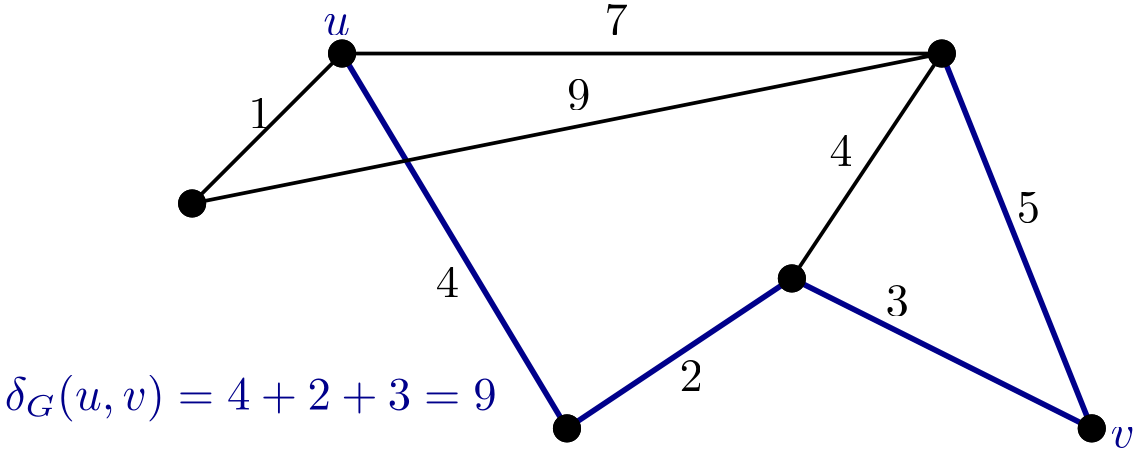
\includegraphics[width=0.75\textwidth]{images/wiener_index.png} % Replace with your own
	\end{center}
\end{frame}

\begin{frame}{Problem Statement: Geometric Spanning Trees}
	\textbf{Reference:} WADS 2023 ~\cite{article:geometric_spanning_trees_minimizing_wiener_index}

	\begin{enumerate}
		\item Input: A set $P$ of $n$ points in the plane.
		      \pause
		\item Goal: Construct a \textbf{spanning tree} on $P$ that minimizes the \textbf{Wiener index}.
		      \pause
		\item The weight function is defined as the Euclidean distance between points.
	\end{enumerate}
\end{frame}

\begin{frame}{Results Summary: Geometric Spanning Trees}
	\begin{itemize}
		\item Spanning tree of $P$ that minimizes the Wiener index is planar.
		      \pause
		\item When $P$ is in convex position, this can be solved in polynomial time.
		      \pause
		\item The hamiltonian path of $P$ that minimizes the Wiener index is not necessarily planar.
		      \pause
		\item Computing such a hamiltonian path is NP-Hard.
	\end{itemize}
\end{frame}

\begin{frame}{Minimum Spanning Tree (MST)}
	\begin{block}{Minimum Spanning Tree (MST)}
		A \textbf{minimum spanning tree} of a weighted undirected graph is a spanning tree that has the minimum total edge weight.
		\begin{itemize}
			\item The MST connects all vertices with the minimum total edge weight.
			\item It is unique if all edge weights are distinct.
		\end{itemize}
	\end{block}
\end{frame}

\section{Approximation Algorithm for Hamiltonian Paths}

\begin{frame}{Divide and Conquer Algorithm for Approximating Hamiltonian Paths}
	\begin{algorithm}[H]
		\caption{DivideAndConquerWiener($P$)}
		\begin{algorithmic}[1]
			\Procedure{DivideAndConquerWiener}{$P$, $depth = 0$, $maxDepth = 10$}
			\If{$|P| \leq 4$ or $depth > maxDepth$}
			\State \Return \Call{BruteForceHamiltonianPath}{$P$}
			\EndIf
			\State $(a, b, c) \gets$ \Call{FindBisectingLine}{$P$}
			\State $(P_L, P_R) \gets$ \Call{PartitionPoints}{$P$, $a$, $b$, $c$}
			\State $\pi_L \gets$ \Call{DivideAndConquerWiener}{$P_L$, $depth+1$}
			\State $\pi_R \gets$ \Call{DivideAndConquerWiener}{$P_R$, $depth+1$}
			\State \Return \Call{ConnectPaths}{$\pi_L$, $\pi_R$}
			\EndProcedure
		\end{algorithmic}
	\end{algorithm}
\end{frame}

\begin{frame}{Supporting Procedure: FindBisectingLine}
	\begin{algorithm}[H]
		\caption{FindBisectingLine($P$)}
		\begin{algorithmic}[1]
			\Procedure{FindBisectingLine}{$P$}
			\State $minX \gets \min_{p \in P} p.x$, $maxX \gets \max_{p \in P} p.x$
			\State $minY \gets \min_{p \in P} p.y$, $maxY \gets \max_{p \in P} p.y$
			\State $width \gets maxX - minX$, $height \gets maxY - minY$
			\If{$width \geq height$}
			\State $midX \gets (minX + maxX)/2$
			\State \Return $(1.0, 0.0, -midX)$ \Comment{Vertical line: $x = midX$}
			\Else
			\State $midY \gets (minY + maxY)/2$
			\State \Return $(0.0, 1.0, -midY)$ \Comment{Horizontal line: $y = midY$}
			\EndIf
			\EndProcedure
		\end{algorithmic}
	\end{algorithm}
\end{frame}

\begin{frame}{Supporting Procedure: PartitionPoints}
	\begin{algorithm}[H]
		\caption{PartitionPoints($P$, $a$, $b$, $c$)}
		\begin{algorithmic}[1]
			\Procedure{PartitionPoints}{$P$, $a$, $b$, $c$}
			\State $L \gets [\ ]$, $R \gets [\ ]$
			\For{each $p \in P$}
			\State $v \gets ap.x + bp.y + c$
			\If{$v \leq 0$}
			\State $L \gets L \cup \{p\}$
			\Else
			\State $R \gets R \cup \{p\}$
			\EndIf
			\EndFor
			\If{$L = \emptyset$}
			\State Move one point from $R$ to $L$
			\ElsIf{$R = \emptyset$}
			\State Move one point from $L$ to $R$
			\EndIf
			\State \Return $(L, R)$
			\EndProcedure
		\end{algorithmic}
	\end{algorithm}
\end{frame}

\begin{frame}{Supporting Procedure: ConnectPaths}
	\begin{algorithm}[H]
		\caption{ConnectPaths($\pi_1$, $\pi_2$)}
		\begin{algorithmic}[1]
			\Procedure{ConnectPaths}{$\pi_1$, $\pi_2$}
			\State $options \gets$ empty list
			\State Append $(\pi_1 + \pi_2, W(\pi_1 + \pi_2))$ to $options$
			\State Append $(\pi_1 + \text{reverse}(\pi_2), W(\pi_1 + \text{reverse}(\pi_2)))$ to $options$
			\State Append $(\text{reverse}(\pi_1) + \pi_2, W(\text{reverse}(\pi_1) + \pi_2))$ to $options$
			\State Append $(\text{reverse}(\pi_1) + \text{reverse}(\pi_2), W(\text{reverse}(\pi_1) + \text{reverse}(\pi_2)))$ to $options$
			\State \Return path with minimum Wiener index from $options$
			\EndProcedure
		\end{algorithmic}
	\end{algorithm}
\end{frame}

\begin{frame}{Approximation Quality and Efficiency}
	\scriptsize
	\begin{table}[htbp]
		\centering
		\begin{tabular}{|c|c|c|c|c|}
			\hline
			\textbf{\#Pts} & \textbf{Approx Ratio} & \textbf{Range}   & \textbf{D\&C Time (s)} & \textbf{Speedup} \\
			\hline
			6              & 1.0206 $\pm$ 0.0501   & [1.0000, 1.3021] & 0.0001                 & 72.4x            \\
			7              & 1.0212 $\pm$ 0.0480   & [1.0000, 1.3014] & 0.0001                 & 481.8x           \\
			8              & 1.0427 $\pm$ 0.0731   & [1.0000, 1.3307] & 0.0002                 & 2800.6x          \\
			9              & 1.0625 $\pm$ 0.0873   & [1.0000, 1.3318] & 0.0003                 & 6785.5x          \\
			10             & 1.0520 $\pm$ 0.0776   & [1.0000, 1.4271] & 0.0003                 & 80249.2x         \\
			\hline
		\end{tabular}
		\caption{Approximation quality and speed comparison with optimal algorithm.}
	\end{table}
\end{frame}

\begin{frame}[allowframebreaks]{References}
	\bibliography{references}
\end{frame}

\begin{frame}
	\begin{center}
		The end.

		\email
	\end{center}
\end{frame}

\end{document}

